% ============================================================================
% Parte 06 — Stewart, Precálculo 7.ª ed., §2.6 "Transformaciones de funciones"
% (pp. 198–209).
%
% Ejercicios elegidos (15) y página del libro:
%   Ej. 11 (p. 206) — Describir transformaciones (desplazamientos combinados)
%   Ej. 17 (p. 206) — Describir transformaciones (estiramiento/reducción horizontal)
%   Ej. 21 (p. 206) — Describir transformaciones de g a partir de f
%   Ej. 23 (p. 206) — Trazar transformaciones de y = x^2
%   Ej. 27 (p. 206) — Identificar transformaciones (gráfica dada I–IV)
%   Ej. 45 (p. 207) — Trazar y = (x-3)^2 + 5
%   Ej. 47 (p. 207) — Trazar y = 3 - (1/2)(x-1)^2 (reflexión en el eje x)
%   Ej. 51 (p. 207) — Trazar y = (1/2)sqrt(x+4) - 3
%   Ej. 61 (p. 207) — Encontrar la ecuación de la gráfica transformada
%   Ej. 63 (p. 207) — Encontrar fórmula desde la gráfica (parábola)
%   Ej. 67 (p. 207) — Encontrar fórmula desde la gráfica (raíz cuadrada)
%   Ej. 71 (p. 208) — Transformaciones a partir de una gráfica dada (a–f)
%   Ej. 87 (p. 208) — Función par o impar (algebraico, f(-x))
%   Ej. 91 (p. 208) — Completar una gráfica para que sea par y para que sea impar
%   Ej. 97 (p. 209) — Aplicación: salto bungee (desplazamiento vertical)
%
% Figuras extraídas del PDF (images/):
%   fig_p06_27.png, fig_p06_63.png, fig_p06_67.png,
%   fig_p06_71.png, fig_p06_91.png, fig_p06_97.png
% El resto de las gráficas se trazan con pgfplots.
% ============================================================================
\documentclass[11pt]{article}
\usepackage[utf8]{inputenc}
\usepackage[spanish]{babel}
\usepackage[margin=2.3cm]{geometry}
\usepackage{amsmath,amssymb}
\usepackage{enumitem}
\usepackage{tcolorbox}
\tcbuselibrary{skins,breakable}
\usepackage{pgfplots}
\pgfplotsset{compat=1.18}
\usepackage{tikz}
\usepackage{graphicx}
\usepackage{array}
\usepackage[hidelinks]{hyperref}

% Notación española opcional (descomenta si quieres \sen en lugar de \sin)
% \DeclareMathOperator{\sen}{sen}
% \DeclareMathOperator{\tg}{tg}
% \DeclareMathOperator{\ctg}{ctg}

\newtcolorbox{sol}{colback=blue!5,colframe=blue!50!black,title=Solución paso a paso,breakable}
\newtcolorbox{teo}{colback=orange!8,colframe=orange!70!black,title=Teoría,breakable}
\newtcolorbox{nota}{colback=green!5,colframe=green!50!black,title=Idea clave,breakable}
\newtcolorbox{tip}{colback=yellow!10,colframe=yellow!60!black,title=Consejo,breakable}
\newtcolorbox{resp}{colback=red!5,colframe=red!50!black,title=Respuesta,breakable}
\newtcolorbox{reg}{colback=red!5,colframe=red!60!black,title=Regla,breakable}
\newtcolorbox{paso}[1]{colback=gray!5,colframe=gray!50!black,title={#1},breakable}

\graphicspath{{../images/}{images/}}
\newcommand{\sen}{\operatorname{sen}}

% babel spanish activa < y > y rompe TikZ/pgfplots (->, >=stealth)
\AtBeginDocument{\shorthandoff{<>}}

\begin{document}
\shorthandoff{<>}  % babel-spanish hace activos < y >; tikz/pgfplots los necesitan literales

\section*{Parte 06 — Transformaciones de funciones (Stewart §2.6, pp. 198--209)}

\begin{teo}
\textbf{Método de la sección 2.6.} Con $c>0$ y partiendo de la gráfica de $y=f(x)$:
\begin{enumerate}[leftmargin=*]
\item \textbf{Desplazamiento vertical.} $y=f(x)+c$ sube $c$ unidades; $y=f(x)-c$ baja $c$ unidades. Se le suma $c$ a la \emph{salida}, así que cada punto se mueve en $y$.
\item \textbf{Desplazamiento horizontal.} $y=f(x-c)$ desplaza $c$ unidades a la \textbf{derecha}; $y=f(x+c)$, $c$ unidades a la \textbf{izquierda}. Va al revés del signo porque para obtener la misma salida hay que \emph{entrar} con un $x$ mayor en $c$.
\item \textbf{Reflexiones.} $y=-f(x)$ refleja en el eje $x$ (cambia el signo de la salida); $y=f(-x)$ refleja en el eje $y$ (cambia el signo de la entrada).
\item \textbf{Estiramiento y reducción verticales.} $y=c\,f(x)$ con $c>1$ estira verticalmente en un factor $c$; con $0<c<1$ reduce (aplasta) en ese factor. Multiplica la salida.
\item \textbf{Estiramiento y reducción horizontales.} $y=f(cx)$ con $c>1$ \textbf{comprime} horizontalmente en un factor $1/c$; con $0<c<1$ \textbf{estira} en un factor $1/c$. Multiplica la entrada, por eso el efecto es el recíproco.
\item \textbf{Orden.} Aplicá las transformaciones en el orden en que están escritas de adentro hacia afuera del argumento, y en el orden que dicte el enunciado cuando este lo fije.
\end{enumerate}
\end{teo}

\begin{tip}
Lo que se repite en toda la sección:
\begin{itemize}[leftmargin=*]
\item \textbf{Regla del punto.} Si $(a,b)$ está en la gráfica de $f$, entonces en $y=k\,f(m(x-h))+v$ está el punto $\left(\dfrac{a}{m}+h,\; k\,b+v\right)$. Con esto basta transformar los puntos clave (vértices, extremos, cortes).
\item \textbf{Funciones estándar del libro:} $y=x^2$ (vértice $(0,0)$), $y=x^3$, $y=|x|$ (vértice $(0,0)$), $y=\sqrt{x}$ (extremo $(0,0)$, solo $x\ge0$), $y=\sqrt[3]{x}$.
\item \textbf{Paridad.} $f$ es \textbf{par} si $f(-x)=f(x)$ (gráfica simétrica respecto al eje $y$); es \textbf{impar} si $f(-x)=-f(x)$ (gráfica simétrica respecto al origen). Si no se cumple ninguna, no es par ni impar.
\item \textbf{Potencias de $-x$:} $(-x)^n=x^n$ si $n$ es par y $(-x)^n=-x^n$ si $n$ es impar. $|-x|=|x|$.
\end{itemize}
\end{tip}

% ===========================================================================
\subsection*{Ejercicio 11 — Describir desplazamientos combinados}

\begin{quote}
\textbf{7--18 $\blacksquare$ Describir transformaciones}\quad Suponga que se da la gráfica de $f$. Describa la forma en que la gráfica de cada función se puede obtener a partir de la gráfica de $f$.

\textbf{11.} \textbf{\textit{a}}) $y=f(x-5)+2$ \hfill \textbf{\textit{b}}) $y=f(x+1)-1$
\end{quote}

\begin{paso}{Paso 1 --- Separar el efecto sobre la entrada y sobre la salida en \textit{a})}
\textbf{Qué hago:} en $y=f(x-5)+2$ leo el $-5$ dentro del argumento (entrada) y el $+2$ fuera (salida).

\textbf{¿De dónde sale?} Del enunciado; el argumento de $f$ es $x-5$ y el término añadido después de evaluar es $+2$.

\textbf{¿Por qué?} Las transformaciones del argumento son horizontales y las de la salida son verticales; son independientes y se pueden aplicar por separado.
\end{paso}

\begin{paso}{Paso 2 --- Traducir cada efecto a un movimiento}
\textbf{Qué hago:} $f(x-5)$ desplaza 5 unidades a la \emph{derecha} y $+2$ sube 2 unidades.

\textbf{¿De dónde sale?} Del paso 1, con la regla $y=f(x-c)\Rightarrow$ derecha $c$, y $y=f(x)+c\Rightarrow$ arriba $c$, con $c=5$ y $c=2$.

\textbf{¿Por qué?} Regla de desplazamiento horizontal y vertical de la sección 2.6: el signo menos en el argumento mueve hacia la derecha, porque hay que entrar con $x$ cinco unidades mayor para reproducir la misma salida.
\end{paso}

\begin{paso}{Paso 3 --- Repetir la lectura en \textit{b})}
\textbf{Qué hago:} en $y=f(x+1)-1$ escribo $x+1=x-(-1)$ y leo el $-1$ exterior.

\textbf{¿De dónde sale?} Del enunciado, reescribiendo el argumento para dejarlo en la forma $x-c$.

\textbf{¿Por qué?} Con $c=-1$ la misma regla da desplazamiento de 1 unidad a la izquierda, y el $-1$ exterior baja 1 unidad.
\end{paso}

\begin{resp}
\textbf{a)} Desplazar la gráfica de $f$ \textbf{5 unidades a la derecha} y \textbf{2 unidades hacia arriba}.\\
\textbf{b)} Desplazar la gráfica de $f$ \textbf{1 unidad a la izquierda} y \textbf{1 unidad hacia abajo}.
\end{resp}

% ===========================================================================
\subsection*{Ejercicio 17 — Estiramiento y reducción horizontales}

\begin{quote}
\textbf{17.} \textbf{\textit{a}}) $y=f(4x)$ \hfill \textbf{\textit{b}}) $y=f\!\left(\tfrac14 x\right)$
\end{quote}

\begin{paso}{Paso 1 --- Reconocer que el factor está en la entrada}
\textbf{Qué hago:} identifico que en ambos casos $x$ aparece multiplicado \emph{dentro} de $f$.

\textbf{¿De dónde sale?} Del enunciado: los argumentos son $4x$ y $\tfrac14x$.

\textbf{¿Por qué?} Multiplicar la entrada produce transformaciones \emph{horizontales}; multiplicar la salida ($c\,f(x)$) produciría verticales.
\end{paso}

\begin{paso}{Paso 2 --- Aplicar la regla del punto}
\textbf{Qué hago:} si $(a,b)$ está en la gráfica de $f$, en $y=f(4x)$ está $\left(\tfrac{a}{4},b\right)$ y en $y=f\!\left(\tfrac14x\right)$ está $(4a,b)$.

\textbf{¿De dónde sale?} De resolver $4x=a$ y $\tfrac14x=a$ para $x$: la abscisa se divide entre el factor.

\textbf{¿Por qué?} La ordenada no cambia porque $f$ devuelve el mismo valor $b$; solo cambia la abscisa que hay que ingresar.
\end{paso}

\begin{paso}{Paso 3 --- Nombrar cada efecto}
\textbf{Qué hago:} concluyo que $c=4>1$ acerca los puntos al eje $y$ (compresión de factor $\tfrac14$) y $c=\tfrac14<1$ los aleja (estiramiento de factor 4).

\textbf{¿De dónde sale?} Del paso 2: las abscisas se multiplican por $\tfrac14$ y por $4$ respectivamente.

\textbf{¿Por qué?} Regla de estiramiento y reducción horizontales: el efecto es el recíproco del factor que multiplica a $x$.
\end{paso}

\begin{resp}
\textbf{a)} \textbf{Reducir (comprimir) horizontalmente} la gráfica de $f$ en un factor de $\tfrac14$.\\
\textbf{b)} \textbf{Estirar horizontalmente} la gráfica de $f$ en un factor de $4$.
\end{resp}

% ===========================================================================
\subsection*{Ejercicio 21 — Describir cómo se obtiene $g$ a partir de $f$}

\begin{quote}
\textbf{19--22 $\blacksquare$ Describir transformaciones}\quad Explique cómo se obtiene la gráfica de $g$ a partir de la gráfica de $f$.

\textbf{21.} \textbf{\textit{a}}) $f(x)=|x|$, \quad $g(x)=|x+2|-2$\\
\phantom{\textbf{21.}} \textbf{\textit{b}}) $f(x)=|x|$, \quad $g(x)=|x-2|+2$
\end{quote}

\begin{paso}{Paso 1 --- Escribir $g$ en la forma $f(x-c)+v$}
\textbf{Qué hago:} reescribo \textbf{a)} como $g(x)=f(x+2)-2$ y \textbf{b)} como $g(x)=f(x-2)+2$.

\textbf{¿De dónde sale?} De sustituir $f(u)=|u|$ con $u=x+2$ y $u=x-2$ en las expresiones del enunciado.

\textbf{¿Por qué?} Reconocer la forma $f(x-c)+v$ es lo que permite aplicar directamente las reglas de desplazamiento.
\end{paso}

\begin{paso}{Paso 2 --- Leer los desplazamientos}
\textbf{Qué hago:} en \textbf{a)} el $+2$ interior mueve 2 a la izquierda y el $-2$ exterior baja 2; en \textbf{b)} el $-2$ interior mueve 2 a la derecha y el $+2$ exterior sube 2.

\textbf{¿De dónde sale?} Del paso 1, con $c=-2,\,v=-2$ y $c=2,\,v=2$.

\textbf{¿Por qué?} Reglas de desplazamiento horizontal ($f(x-c)$ va a la derecha si $c>0$) y vertical de la sección 2.6.
\end{paso}

\begin{paso}{Paso 3 --- Verificar con el vértice}
\textbf{Qué hago:} el vértice $(0,0)$ de $y=|x|$ va a $(-2,-2)$ en \textbf{a)} y a $(2,2)$ en \textbf{b)}.

\textbf{¿De dónde sale?} De la regla del punto aplicada a $(0,0)$ con los desplazamientos del paso 2.

\textbf{¿Por qué?} Comprobación directa: $g(-2)=|-2+2|-2=-2$ y $g(2)=|2-2|+2=2$, que es donde el valor absoluto alcanza su valor extremo.
\end{paso}

\begin{resp}
\textbf{a)} Desplazar $y=|x|$ \textbf{2 unidades a la izquierda} y \textbf{2 hacia abajo} (vértice en $(-2,-2)$).\\
\textbf{b)} Desplazar $y=|x|$ \textbf{2 unidades a la derecha} y \textbf{2 hacia arriba} (vértice en $(2,2)$).
\end{resp}

% ===========================================================================
\subsection*{Ejercicio 23 — Trazar transformaciones de $y=x^2$}

\begin{quote}
\textbf{23. Trazar gráficas de transformaciones}\quad Use la gráfica de $y=x^2$ de la figura 4 para trazar la gráfica de lo siguiente.

\textbf{\textit{a}}) $g(x)=x^2+1$ \hfill \textbf{\textit{b}}) $g(x)=(x-1)^2$\\
\textbf{\textit{c}}) $g(x)=-x^2$ \hfill \textbf{\textit{d}}) $g(x)=(x-1)^2+3$
\end{quote}

\begin{paso}{Paso 1 --- Clasificar cada transformación}
\textbf{Qué hago:} leo el tipo de cada una: \textbf{a)} $+1$ fuera, \textbf{b)} $-1$ dentro, \textbf{c)} signo menos fuera, \textbf{d)} $-1$ dentro y $+3$ fuera.

\textbf{¿De dónde sale?} De la posición del número respecto al cuadrado en cada fórmula del enunciado.

\textbf{¿Por qué?} Dentro del argumento $\Rightarrow$ horizontal; fuera $\Rightarrow$ vertical; signo menos fuera $\Rightarrow$ reflexión en el eje $x$.
\end{paso}

\begin{paso}{Paso 2 --- Mover el vértice $(0,0)$ de $y=x^2$}
\textbf{Qué hago:} aplico la regla del punto al vértice: \textbf{a)} $(0,1)$; \textbf{b)} $(1,0)$; \textbf{c)} $(0,0)$ pero abriendo hacia abajo; \textbf{d)} $(1,3)$.

\textbf{¿De dónde sale?} Del paso 1: subir 1; derecha 1; reflejar; derecha 1 y arriba 3.

\textbf{¿Por qué?} La forma de la parábola no cambia (no hay factores multiplicando), así que basta reubicar el vértice y conservar la abertura.
\end{paso}

\begin{paso}{Paso 3 --- Trazar}
\textbf{Qué hago:} dibujo las cuatro parábolas con la misma abertura que $y=x^2$ (punteada como referencia).

\textbf{¿De dónde sale?} De los vértices del paso 2.

\textbf{¿Por qué?} Desplazar y reflejar son isometrías de la gráfica: preservan la forma.

\begin{center}
\begin{tikzpicture}
\begin{axis}[name=a, axis lines=middle, xlabel={$x$}, ylabel={$y$},
  xmin=-3.2,xmax=3.2, ymin=-2.5,ymax=6.5, width=6.6cm,height=5cm,
  grid=both, grid style={gray!20}, title={\small a) $g(x)=x^2+1$}]
  \addplot[dashed,gray,domain=-2.4:2.4,samples=60]{x^2};
  \addplot[thick,blue,domain=-2.4:2.4,samples=60]{x^2+1};
  \addplot[only marks,mark=*,red] coordinates {(0,1)};
\end{axis}
\begin{axis}[name=b, at={(a.east)}, anchor=west, xshift=0.6cm,
  axis lines=middle, xlabel={$x$}, ylabel={$y$},
  xmin=-2.2,xmax=4.2, ymin=-2.5,ymax=6.5, width=6.6cm,height=5cm,
  grid=both, grid style={gray!20}, title={\small b) $g(x)=(x-1)^2$}]
  \addplot[dashed,gray,domain=-2.2:2.4,samples=60]{x^2};
  \addplot[thick,blue,domain=-1.4:3.4,samples=60]{(x-1)^2};
  \addplot[only marks,mark=*,red] coordinates {(1,0)};
\end{axis}
\begin{axis}[name=c, at={(a.south)}, anchor=north, yshift=-0.8cm,
  axis lines=middle, xlabel={$x$}, ylabel={$y$},
  xmin=-3.2,xmax=3.2, ymin=-6.5,ymax=6.5, width=6.6cm,height=5cm,
  grid=both, grid style={gray!20}, title={\small c) $g(x)=-x^2$}]
  \addplot[dashed,gray,domain=-2.4:2.4,samples=60]{x^2};
  \addplot[thick,blue,domain=-2.4:2.4,samples=60]{-x^2};
  \addplot[only marks,mark=*,red] coordinates {(0,0)};
\end{axis}
\begin{axis}[name=d, at={(c.east)}, anchor=west, xshift=0.6cm,
  axis lines=middle, xlabel={$x$}, ylabel={$y$},
  xmin=-2.2,xmax=4.2, ymin=-1.5,ymax=8.5, width=6.6cm,height=5cm,
  grid=both, grid style={gray!20}, title={\small d) $g(x)=(x-1)^2+3$}]
  \addplot[dashed,gray,domain=-2.2:2.4,samples=60]{x^2};
  \addplot[thick,blue,domain=-1.2:3.2,samples=60]{(x-1)^2+3};
  \addplot[only marks,mark=*,red] coordinates {(1,3)};
\end{axis}
\end{tikzpicture}
\end{center}
\end{paso}

\begin{resp}
\textbf{a)} $y=x^2$ subida 1 unidad; vértice $(0,1)$.\quad
\textbf{b)} $y=x^2$ desplazada 1 unidad a la derecha; vértice $(1,0)$.\\
\textbf{c)} $y=x^2$ reflejada en el eje $x$; vértice $(0,0)$, abre hacia abajo.\quad
\textbf{d)} $y=x^2$ desplazada 1 a la derecha y 3 hacia arriba; vértice $(1,3)$.
\end{resp}

% ===========================================================================
\subsection*{Ejercicio 27 — Identificar la transformación en una gráfica dada}

\begin{quote}
\textbf{25--28 $\blacksquare$ Identificar transformaciones}\quad Relacione la gráfica con la función. (Vea la gráfica de $y=|x|$ en la página 96.)

\textbf{27.} $y=|x|-1$
\begin{center}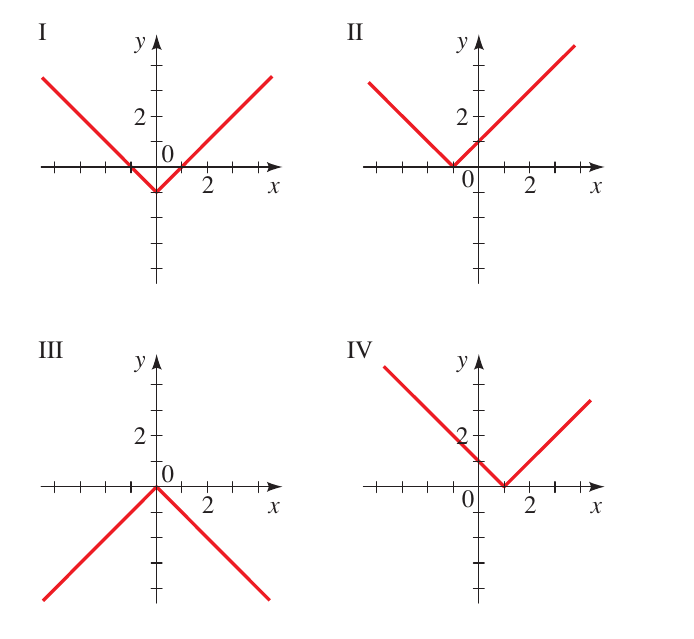
\includegraphics[width=0.62\textwidth]{fig_p06_27.png}\end{center}
\end{quote}

\begin{paso}{Paso 1 --- Predecir el vértice antes de mirar las gráficas}
\textbf{Qué hago:} aplico la regla del punto al vértice $(0,0)$ de $y=|x|$: el $-1$ está fuera del valor absoluto, así que el vértice baja a $(0,-1)$.

\textbf{¿De dónde sale?} Del enunciado $y=|x|-1$, donde el $-1$ actúa sobre la salida.

\textbf{¿Por qué?} Regla de desplazamiento vertical: restar una constante baja la gráfica sin moverla lateralmente.
\end{paso}

\begin{paso}{Paso 2 --- Buscar en I--IV el vértice $(0,-1)$ con abertura hacia arriba}
\textbf{Qué hago:} descarto III (abre hacia abajo, vértice $(0,0)$: es $y=-|x|$), II (vértice $(-1,0)$: es $y=|x+1|$) y IV (vértice $(1,0)$: es $y=|x-1|$).

\textbf{¿De dónde sale?} De leer el vértice de cada gráfica de la figura.

\textbf{¿Por qué?} El vértice determina de forma única la traslación, y el sentido de abertura indica si hubo reflexión en el eje $x$.
\end{paso}

\begin{resp}
$y=|x|-1$ corresponde a la gráfica \textbf{I} (vértice en $(0,-1)$, abre hacia arriba).
\end{resp}

% ===========================================================================
\subsection*{Ejercicio 45 — Trazar $y=(x-3)^2+5$}

\begin{quote}
\textbf{29--52 $\blacksquare$ Trazar transformaciones de gráficas}\quad Trace la gráfica de la función no colocando los puntos sino empezando con la gráfica de una función estándar y aplique las transformaciones.

\textbf{45.} $y=(x-3)^2+5$
\end{quote}

\begin{paso}{Paso 1 --- Identificar la función estándar}
\textbf{Qué hago:} tomo $f(x)=x^2$ como base y escribo $y=f(x-3)+5$.

\textbf{¿De dónde sale?} Del enunciado: la expresión es un cuadrado perfecto de $x-3$ más 5.

\textbf{¿Por qué?} La gráfica de $y=x^2$ es una de las funciones estándar del libro, y el resto es una traslación.
\end{paso}

\begin{paso}{Paso 2 --- Aplicar los dos desplazamientos}
\textbf{Qué hago:} desplazo 3 unidades a la derecha (por $x-3$) y luego 5 hacia arriba (por $+5$); el vértice $(0,0)$ va a $(3,5)$.

\textbf{¿De dónde sale?} Del paso 1, con $c=3$ y $v=5$.

\textbf{¿Por qué?} Reglas de desplazamiento horizontal y vertical; el orden entre ellas no altera el resultado porque una mueve solo $x$ y la otra solo $y$.

\begin{center}
\begin{tikzpicture}
\begin{axis}[axis lines=middle, xlabel={$x$}, ylabel={$y$},
  xmin=-2.5,xmax=7, ymin=-1,ymax=11, width=9.5cm,height=6cm,
  grid=both, grid style={gray!20}, xtick={-2,-1,...,6}, ytick={0,2,...,10}]
  \addplot[dashed,gray,domain=-2.4:2.4,samples=60]{x^2};
  \addplot[thick,blue,domain=0.6:5.4,samples=60]{(x-3)^2+5};
  \addplot[only marks,mark=*,red] coordinates {(3,5)};
  \node[anchor=south west,font=\small] at (axis cs:3,5) {$(3,5)$};
\end{axis}
\end{tikzpicture}
\end{center}
\end{paso}

\begin{resp}
Parábola con la misma abertura que $y=x^2$, \textbf{vértice $(3,5)$}, abierta hacia arriba; no corta al eje $x$ porque $(x-3)^2+5\ge 5>0$.
\end{resp}

% ===========================================================================
\subsection*{Ejercicio 47 — Reducción vertical y reflexión: $y=3-\tfrac12(x-1)^2$}

\begin{quote}
\textbf{47.} $y=3-\tfrac12(x-1)^2$
\end{quote}

\begin{paso}{Paso 1 --- Ordenar la expresión para leer las transformaciones}
\textbf{Qué hago:} reescribo $y=-\tfrac12(x-1)^2+3$ y tomo $f(x)=x^2$ como base.

\textbf{¿De dónde sale?} Del enunciado, conmutando los sumandos.

\textbf{¿Por qué?} En la forma $y=k\,f(x-c)+v$ cada constante corresponde a una única transformación, lo que evita confundir el $3$ con un desplazamiento horizontal.
\end{paso}

\begin{paso}{Paso 2 --- Aplicar las transformaciones en orden}
\textbf{Qué hago:} (i) $x-1$: 1 unidad a la derecha; (ii) factor $\tfrac12$: reducción vertical de factor $\tfrac12$; (iii) signo menos: reflexión en el eje $x$; (iv) $+3$: 3 unidades hacia arriba.

\textbf{¿De dónde sale?} De las cuatro constantes de la forma del paso 1: $c=1$, $|k|=\tfrac12$, $\operatorname{signo}(k)=-$, $v=3$.

\textbf{¿Por qué?} Reglas de desplazamiento, de reducción vertical ($0<|k|<1$ aplasta) y de reflexión en el eje $x$ ($k<0$).
\end{paso}

\begin{paso}{Paso 3 --- Ubicar el vértice y un par de puntos de control}
\textbf{Qué hago:} el vértice $(0,0)$ va a $(1,3)$; el punto $(2,4)$ de $y=x^2$ va a $x=1+2=3$, $y=-\tfrac12(4)+3=1$.

\textbf{¿De dónde sale?} De la regla del punto: $(a,b)\mapsto (a+1,\,-\tfrac12 b+3)$.

\textbf{¿Por qué?} Dos o tres puntos transformados fijan la abertura de la parábola sin tabular.

\begin{center}
\begin{tikzpicture}
\begin{axis}[axis lines=middle, xlabel={$x$}, ylabel={$y$},
  xmin=-3,xmax=5.5, ymin=-4,ymax=6, width=9.5cm,height=6cm,
  grid=both, grid style={gray!20}, xtick={-3,-2,...,5}, ytick={-4,-2,0,2,4,6}]
  \addplot[dashed,gray,domain=-2.2:2.2,samples=60]{x^2};
  \addplot[thick,blue,domain=-2.7:4.7,samples=80]{3-0.5*(x-1)^2};
  \addplot[only marks,mark=*,red] coordinates {(1,3) (3,1) (-1,1)};
  \node[anchor=south,font=\small] at (axis cs:1,3) {$(1,3)$};
\end{axis}
\end{tikzpicture}
\end{center}
\end{paso}

\begin{resp}
Parábola \textbf{abierta hacia abajo}, más ancha que $y=x^2$ (factor $\tfrac12$), con \textbf{vértice $(1,3)$}; pasa por $(-1,1)$ y $(3,1)$.
\end{resp}

% ===========================================================================
\subsection*{Ejercicio 51 — Trazar $y=\tfrac12\sqrt{x+4}-3$}

\begin{quote}
\textbf{51.} $y=\tfrac12\sqrt{x+4}-3$
\end{quote}

\begin{paso}{Paso 1 --- Identificar la base y las tres transformaciones}
\textbf{Qué hago:} tomo $f(x)=\sqrt{x}$ y escribo $y=\tfrac12 f(x+4)-3$.

\textbf{¿De dónde sale?} Del enunciado: radicando $x+4$, factor exterior $\tfrac12$, término $-3$.

\textbf{¿Por qué?} $y=\sqrt{x}$ es función estándar; lo demás son transformaciones ya catalogadas.
\end{paso}

\begin{paso}{Paso 2 --- Aplicarlas al punto inicial y al dominio}
\textbf{Qué hago:} 4 unidades a la izquierda, reducción vertical de factor $\tfrac12$ y 3 unidades hacia abajo; el extremo $(0,0)$ va a $(-4,-3)$ y el dominio pasa de $x\ge0$ a $x\ge-4$.

\textbf{¿De dónde sale?} De la regla del punto $(a,b)\mapsto(a-4,\tfrac12 b-3)$ y de exigir $x+4\ge0$.

\textbf{¿Por qué?} La raíz de índice par solo está definida para radicando no negativo, y el desplazamiento horizontal arrastra también al dominio.
\end{paso}

\begin{paso}{Paso 3 --- Puntos de control y trazo}
\textbf{Qué hago:} transformo $(4,2)$ y $(16,4)$ de $y=\sqrt x$: dan $(0,-2)$ y $(12,-1)$.

\textbf{¿De dónde sale?} De la misma regla del punto del paso 2.

\textbf{¿Por qué?} Fijan la rapidez de crecimiento de la curva, que es la mitad de la de $\sqrt x$.

\begin{center}
\begin{tikzpicture}
\begin{axis}[axis lines=middle, xlabel={$x$}, ylabel={$y$},
  xmin=-6,xmax=14, ymin=-4.5,ymax=2, width=10.5cm,height=5.5cm,
  grid=both, grid style={gray!20}, xtick={-4,-2,...,12}, ytick={-4,-3,...,1}]
  \addplot[dashed,gray,domain=0:12,samples=80]{sqrt(x)};
  \addplot[thick,blue,domain=-4:13,samples=100]{0.5*sqrt(x+4)-3};
  \addplot[only marks,mark=*,red] coordinates {(-4,-3) (0,-2) (12,-1)};
  \node[anchor=north west,font=\small] at (axis cs:-4,-3) {$(-4,-3)$};
\end{axis}
\end{tikzpicture}
\end{center}
\end{paso}

\begin{resp}
Media rama de raíz cuadrada que empieza en $(-4,-3)$ y crece hacia la derecha con la mitad de la altura de $\sqrt{x}$. Dominio $[-4,\infty)$, rango $[-3,\infty)$.
\end{resp}

% ===========================================================================
\subsection*{Ejercicio 61 — Encontrar la ecuación de la gráfica transformada}

\begin{quote}
\textbf{53--62 $\blacksquare$ Encontrar ecuaciones para transformaciones}\quad Se da una función $f$ y las transformaciones indicadas se aplican a su gráfica (en el orden dado). Escriba la ecuación para la gráfica final transformada.

\textbf{61.} $f(x)=x^2$; estirar verticalmente en un factor de 2, desplazar hacia abajo 2 unidades y desplazar 3 unidades a la derecha
\end{quote}

\begin{paso}{Paso 1 --- Estiramiento vertical de factor 2}
\textbf{Qué hago:} multiplico la salida por 2: $y=2x^2$.

\textbf{¿De dónde sale?} De la primera transformación del enunciado aplicada a $f(x)=x^2$.

\textbf{¿Por qué?} Regla de estiramiento vertical: $y=c\,f(x)$ con $c=2>1$ duplica cada ordenada.
\end{paso}

\begin{paso}{Paso 2 --- Desplazamiento 2 unidades hacia abajo}
\textbf{Qué hago:} resto 2 a la expresión anterior: $y=2x^2-2$.

\textbf{¿De dónde sale?} Del resultado del paso 1 y de la segunda transformación del enunciado.

\textbf{¿Por qué?} Regla de desplazamiento vertical: restar una constante baja la gráfica.
\end{paso}

\begin{paso}{Paso 3 --- Desplazamiento 3 unidades a la derecha}
\textbf{Qué hago:} reemplazo $x$ por $x-3$ en \emph{toda} la expresión: $y=2(x-3)^2-2$.

\textbf{¿De dónde sale?} Del resultado del paso 2 y de la tercera transformación del enunciado.

\textbf{¿Por qué?} Regla de desplazamiento horizontal: $y=g(x-3)$ mueve la gráfica de $g$ tres unidades a la derecha; solo se sustituye la variable, no el término constante $-2$.
\end{paso}

\begin{resp}
$y=2(x-3)^2-2$ \quad (vértice $(3,-2)$).
\end{resp}

% ===========================================================================
\subsection*{Ejercicio 63 — Encontrar la fórmula de $g$ desde la gráfica}

\begin{quote}
\textbf{63--68 $\blacksquare$ Encontrar fórmulas para transformaciones}\quad Se dan las gráficas de $f$ y de $g$. Encuentre una fórmula para la función $g$.

\textbf{63.}
\begin{center}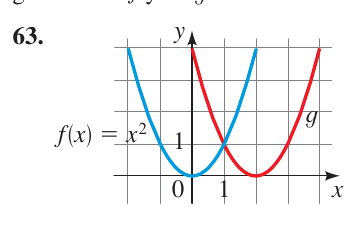
\includegraphics[width=0.44\textwidth]{fig_p06_63.png}\end{center}
\end{quote}

\begin{paso}{Paso 1 --- Comparar forma y abertura}
\textbf{Qué hago:} verifico que $g$ tiene la misma forma y la misma abertura que $f(x)=x^2$, solo corrida.

\textbf{¿De dónde sale?} De la figura: ambas parábolas abren hacia arriba y suben lo mismo por unidad horizontal.

\textbf{¿Por qué?} Si no hay cambio de abertura ni de sentido, la transformación es solo una traslación (sin factores ni reflexiones).
\end{paso}

\begin{paso}{Paso 2 --- Leer el vértice de $g$}
\textbf{Qué hago:} el vértice de $g$ está en $(2,0)$, mientras que el de $f$ está en $(0,0)$; el desplazamiento es 2 unidades a la derecha y 0 verticales.

\textbf{¿De dónde sale?} De la figura: el mínimo de la curva roja está sobre el eje $x$, dos unidades a la derecha del origen.

\textbf{¿Por qué?} El vértice es el punto que identifica la traslación de una parábola.
\end{paso}

\begin{paso}{Paso 3 --- Escribir la fórmula y verificar}
\textbf{Qué hago:} $g(x)=f(x-2)=(x-2)^2$; compruebo con la figura que $g(0)=4$.

\textbf{¿De dónde sale?} Del paso 2 y de la regla $y=f(x-c)$ con $c=2$.

\textbf{¿Por qué?} La curva roja corta al eje $y$ a la altura 4 en la figura, lo que confirma la fórmula.
\end{paso}

\begin{resp}
$g(x)=(x-2)^2$
\end{resp}

% ===========================================================================
\subsection*{Ejercicio 67 — Fórmula de $g$ con reflexión y desplazamiento}

\begin{quote}
\textbf{67.}
\begin{center}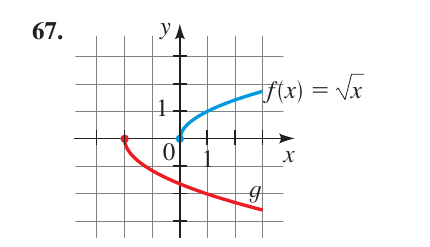
\includegraphics[width=0.46\textwidth]{fig_p06_67.png}\end{center}
\end{quote}

\begin{paso}{Paso 1 --- Detectar la reflexión}
\textbf{Qué hago:} observo que $g$ está por debajo del eje $x$ y \emph{decrece}, mientras $f(x)=\sqrt{x}$ está por encima y crece.

\textbf{¿De dónde sale?} De la figura: la curva roja es la imagen especular de la azul respecto de una recta horizontal.

\textbf{¿Por qué?} Cambiar el signo de la salida, $y=-f(x)$, refleja la gráfica en el eje $x$ e invierte el crecimiento.
\end{paso}

\begin{paso}{Paso 2 --- Leer el desplazamiento horizontal desde el punto extremo}
\textbf{Qué hago:} el extremo de $f$ está en $(0,0)$ y el de $g$ en $(-2,0)$, luego hay 2 unidades a la izquierda y ninguna vertical.

\textbf{¿De dónde sale?} De la figura: el punto marcado de la curva roja está sobre el eje $x$ en $x=-2$.

\textbf{¿Por qué?} El extremo de la rama de raíz cuadrada es el punto que fija la traslación, porque ahí el radicando vale 0.
\end{paso}

\begin{paso}{Paso 3 --- Componer y verificar}
\textbf{Qué hago:} escribo $g(x)=-f(x+2)=-\sqrt{x+2}$ y compruebo un punto: $g(2)=-\sqrt{4}=-2$.

\textbf{¿De dónde sale?} De los pasos 1 y 2: reflexión en el eje $x$ más 2 unidades a la izquierda.

\textbf{¿Por qué?} En la figura, la curva roja pasa cerca de $(2,-2)$, lo que confirma la fórmula; el dominio $x\ge-2$ también coincide.
\end{paso}

\begin{resp}
$g(x)=-\sqrt{x+2}$, \; con dominio $[-2,\infty)$.
\end{resp}

% ===========================================================================
\subsection*{Ejercicio 71 — Transformaciones a partir de una gráfica dada}

\begin{quote}
\textbf{71--74 $\blacksquare$ Transformaciones de gráficas}\quad Se da la gráfica de $f$. Trace las gráficas de las siguientes funciones $f$.

\textbf{71.} \textbf{\textit{a}}) $y=f(x-2)$ \hfill \textbf{\textit{b}}) $y=f(x)-2$\\
\phantom{\textbf{71.}} \textbf{\textit{c}}) $y=2f(x)$ \hfill \textbf{\textit{d}}) $y=-f(x)+3$\\
\phantom{\textbf{71.}} \textbf{\textit{e}}) $y=f(-x)$ \hfill \textbf{\textit{f}}) $y=\tfrac12 f(x-1)$
\begin{center}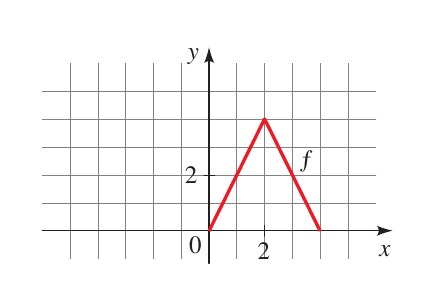
\includegraphics[width=0.42\textwidth]{fig_p06_71.png}\end{center}
\end{quote}

\begin{paso}{Paso 1 --- Extraer los puntos clave de $f$}
\textbf{Qué hago:} leo de la figura los tres vértices de la poligonal: $(0,0)$, $(2,4)$ y $(4,0)$.

\textbf{¿De dónde sale?} De la gráfica dada: la curva sale del origen, sube hasta el pico y vuelve al eje $x$.

\textbf{¿Por qué?} Como $f$ es lineal a trozos, los tres vértices determinan toda la gráfica; transformar la gráfica se reduce a transformar esos tres puntos.
\end{paso}

\begin{paso}{Paso 2 --- Aplicar la regla del punto a cada inciso}
\textbf{Qué hago:} transformo $(a,b)$ según cada fórmula.

\textbf{¿De dónde sale?} De las reglas de la sección aplicadas a los puntos del paso 1.

\textbf{¿Por qué?} Las transformaciones actúan punto a punto, y la poligonal se reconstruye uniendo las imágenes con segmentos.

\begin{center}\small
\begin{tabular}{@{}lll@{}}
\hline
Inciso & Regla sobre $(a,b)$ & Vértices imagen\\
\hline
a) $y=f(x-2)$ & $(a+2,\;b)$ & $(2,0)$, $(4,4)$, $(6,0)$\\
b) $y=f(x)-2$ & $(a,\;b-2)$ & $(0,-2)$, $(2,2)$, $(4,-2)$\\
c) $y=2f(x)$ & $(a,\;2b)$ & $(0,0)$, $(2,8)$, $(4,0)$\\
d) $y=-f(x)+3$ & $(a,\;-b+3)$ & $(0,3)$, $(2,-1)$, $(4,3)$\\
e) $y=f(-x)$ & $(-a,\;b)$ & $(0,0)$, $(-2,4)$, $(-4,0)$\\
f) $y=\tfrac12f(x-1)$ & $(a+1,\;\tfrac12 b)$ & $(1,0)$, $(3,2)$, $(5,0)$\\
\hline
\end{tabular}
\end{center}
\end{paso}

\begin{paso}{Paso 3 --- Trazar las seis poligonales}
\textbf{Qué hago:} uno con segmentos los vértices imagen de cada fila (en gris punteado, $f$ original).

\textbf{¿De dónde sale?} De la tabla del paso 2.

\textbf{¿Por qué?} Las transformaciones consideradas son afines en cada coordenada, así que llevan segmentos en segmentos.

\begin{center}
\begin{tikzpicture}[/pgfplots/every axis/.append style={
  axis lines=middle, xlabel={$x$}, ylabel={$y$},
  width=5.6cm, height=4.3cm, grid=both, grid style={gray!20},
  title style={font=\small}}]
\begin{axis}[name=a, xmin=-1,xmax=7, ymin=-1,ymax=5, title={a) $y=f(x-2)$}]
  \addplot[dashed,gray] coordinates {(0,0) (2,4) (4,0)};
  \addplot[thick,blue] coordinates {(2,0) (4,4) (6,0)};
\end{axis}
\begin{axis}[name=b, at={(a.east)}, anchor=west, xshift=0.7cm,
  xmin=-1,xmax=5, ymin=-3,ymax=5, title={b) $y=f(x)-2$}]
  \addplot[dashed,gray] coordinates {(0,0) (2,4) (4,0)};
  \addplot[thick,blue] coordinates {(0,-2) (2,2) (4,-2)};
\end{axis}
\begin{axis}[name=c, at={(b.east)}, anchor=west, xshift=0.7cm,
  xmin=-1,xmax=5, ymin=-1,ymax=9, title={c) $y=2f(x)$}]
  \addplot[dashed,gray] coordinates {(0,0) (2,4) (4,0)};
  \addplot[thick,blue] coordinates {(0,0) (2,8) (4,0)};
\end{axis}
\begin{axis}[name=d, at={(a.south)}, anchor=north, yshift=-1.35cm,
  xmin=-1,xmax=5, ymin=-2,ymax=5, title={d) $y=-f(x)+3$}]
  \addplot[dashed,gray] coordinates {(0,0) (2,4) (4,0)};
  \addplot[thick,blue] coordinates {(0,3) (2,-1) (4,3)};
\end{axis}
\begin{axis}[name=e, at={(d.east)}, anchor=west, xshift=0.7cm,
  xmin=-5,xmax=5, ymin=-1,ymax=5, title={e) $y=f(-x)$}]
  \addplot[dashed,gray] coordinates {(0,0) (2,4) (4,0)};
  \addplot[thick,blue] coordinates {(0,0) (-2,4) (-4,0)};
\end{axis}
\begin{axis}[name=fx, at={(e.east)}, anchor=west, xshift=0.7cm,
  xmin=-1,xmax=6, ymin=-1,ymax=5, title={f) $y=\frac12 f(x-1)$}]
  \addplot[dashed,gray] coordinates {(0,0) (2,4) (4,0)};
  \addplot[thick,blue] coordinates {(1,0) (3,2) (5,0)};
\end{axis}
\end{tikzpicture}
\end{center}
\end{paso}

\begin{resp}
Poligonales con vértices: \textbf{a)} $(2,0),(4,4),(6,0)$; \textbf{b)} $(0,-2),(2,2),(4,-2)$; \textbf{c)} $(0,0),(2,8),(4,0)$; \textbf{d)} $(0,3),(2,-1),(4,3)$; \textbf{e)} $(0,0),(-2,4),(-4,0)$; \textbf{f)} $(1,0),(3,2),(5,0)$.
\end{resp}

% ===========================================================================
\subsection*{Ejercicio 87 — Función par o impar (algebraicamente)}

\begin{quote}
\textbf{83--90 $\blacksquare$ Funciones pares e impares}\quad Determine si la función $f$ es par, impar o ninguna de estas. Si $f$ es par o impar, use simetría para trazar su gráfica.

\textbf{87.} $f(x)=x^3-x$
\end{quote}

\begin{paso}{Paso 1 --- Calcular $f(-x)$}
\textbf{Qué hago:} sustituyo $-x$ en cada aparición de $x$ y simplifico.

\textbf{¿De dónde sale?} Del enunciado $f(x)=x^3-x$.

\textbf{¿Por qué?} La definición de par e impar se decide comparando $f(-x)$ con $f(x)$ y con $-f(x)$.
\[
f(-x)=(-x)^3-(-x)=-x^3+x
\]
\end{paso}

\begin{paso}{Paso 2 --- Comparar con $f(x)$ y con $-f(x)$}
\textbf{Qué hago:} factorizo el signo: $-x^3+x=-(x^3-x)=-f(x)$.

\textbf{¿De dónde sale?} Del resultado del paso 1, sacando $-1$ como factor común.

\textbf{¿Por qué?} Se cumple $f(-x)=-f(x)$ para todo $x$ real, que es exactamente la definición de función impar.
\end{paso}

\begin{paso}{Paso 3 --- Usar la simetría para trazar}
\textbf{Qué hago:} tabulo solo $x\ge0$ y completo por simetría respecto al origen: $f(0)=0$, $f(1)=0$, $f(2)=6$, y el mínimo local visible cerca de $x\approx0.6$ con $f(0.6)=-0.384$.

\textbf{¿De dónde sale?} De evaluar $f(x)=x^3-x$; las raíces salen de $x^3-x=x(x-1)(x+1)=0$.

\textbf{¿Por qué?} La gráfica de una función impar es simétrica respecto al origen, así que la mitad $x<0$ se obtiene rotando $180^\circ$ la mitad $x\ge0$.

\begin{center}
\begin{tikzpicture}
\begin{axis}[axis lines=middle, xlabel={$x$}, ylabel={$y$},
  xmin=-2.2,xmax=2.2, ymin=-3,ymax=3, width=9cm,height=6cm,
  grid=both, grid style={gray!20}, xtick={-2,-1,0,1,2}, ytick={-3,-2,...,3}]
  \addplot[thick,blue,domain=-1.8:1.8,samples=120]{x^3-x};
  \addplot[only marks,mark=*,red] coordinates {(-1,0) (0,0) (1,0)};
\end{axis}
\end{tikzpicture}
\end{center}
\end{paso}

\begin{resp}
$f$ es \textbf{impar}, porque $f(-x)=-x^3+x=-f(x)$. Su gráfica es simétrica respecto al \textbf{origen} y corta al eje $x$ en $x=-1,0,1$.
\end{resp}

% ===========================================================================
\subsection*{Ejercicio 91 — Completar una gráfica para que sea par y para que sea impar}

\begin{quote}
\textbf{91--92 $\blacksquare$ Trazar gráficas pares e impares}\quad Se da la gráfica de una función definida por $x\ge0$. Complete la gráfica para $x<0$ para que sea \textbf{\textit{a}}) una función par y \textbf{\textit{b}}) una función impar.

\textbf{91.}
\begin{center}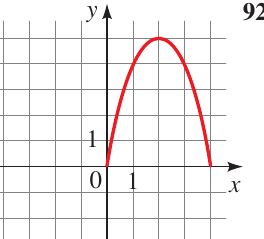
\includegraphics[width=0.34\textwidth]{fig_p06_91.png}\end{center}
\end{quote}

\begin{paso}{Paso 1 --- Traducir cada definición a una construcción geométrica}
\textbf{Qué hago:} para el caso par uso $f(-x)=f(x)$; para el impar, $f(-x)=-f(x)$.

\textbf{¿De dónde sale?} De la definición de función par e impar de la sección 2.6.

\textbf{¿Por qué?} $f(-x)=f(x)$ significa reflejar en el eje $y$ (misma altura); $f(-x)=-f(x)$ significa reflejar en el eje $y$ y además en el eje $x$, es decir, girar $180^\circ$ alrededor del origen.
\end{paso}

\begin{paso}{Paso 2 --- Aplicarlo a los puntos clave del arco dado}
\textbf{Qué hago:} el arco dado va de $(0,0)$ a $(4,0)$ con máximo $\approx(2,5)$; en la parte par esos puntos van a $(0,0)$, $(-4,0)$ y $(-2,5)$; en la impar, a $(0,0)$, $(-4,0)$ y $(-2,-5)$.

\textbf{¿De dónde sale?} De leer la figura y aplicar $(a,b)\mapsto(-a,b)$ y $(a,b)\mapsto(-a,-b)$.

\textbf{¿Por qué?} Son exactamente las dos reglas del paso 1 escritas punto a punto.
\end{paso}

\begin{paso}{Paso 3 --- Trazar las dos completaciones}
\textbf{Qué hago:} dibujo en azul el arco dado y en rojo la parte añadida para $x<0$.

\textbf{¿De dónde sale?} Del paso 2.

\textbf{¿Por qué?} Ambas completaciones son únicas: la condición de paridad determina el valor de $f$ en cada $x<0$ a partir del valor en $-x>0$.

\begin{center}
\begin{tikzpicture}[/pgfplots/every axis/.append style={
  axis lines=middle, xlabel={$x$}, ylabel={$y$},
  width=7.4cm, height=5cm, grid=both, grid style={gray!20},
  xtick={-4,-3,...,4}, title style={font=\small}}]
\begin{axis}[name=par, xmin=-5,xmax=5, ymin=-1,ymax=6, ytick={0,1,...,5},
  title={a) completada como función \emph{par}}]
  \addplot[thick,blue,domain=0:4,samples=120]{5*((x*(4-x)/4)^0.85)};
  \addplot[thick,red,domain=-4:0,samples=120]{5*(((-x)*(4+x)/4)^0.85)};
\end{axis}
\begin{axis}[name=imp, at={(par.east)}, anchor=west, xshift=0.8cm,
  xmin=-5,xmax=5, ymin=-6,ymax=6, ytick={-5,-3,3,5},
  title={b) completada como función \emph{impar}}]
  \addplot[thick,blue,domain=0:4,samples=120]{5*((x*(4-x)/4)^0.85)};
  \addplot[thick,red,domain=-4:0,samples=120]{-5*(((-x)*(4+x)/4)^0.85)};
\end{axis}
\end{tikzpicture}
\end{center}
\end{paso}

\begin{nota}
El arco dado en el libro no tiene fórmula explícita; el trazo de arriba usa una curva con los mismos puntos de paso ($(0,0)$, máximo $\approx(2,5)$ y $(4,0)$) solo para ilustrar. Lo que se evalúa es la construcción: \emph{reflejar en el eje $y$} para la par y \emph{girar $180^\circ$ respecto al origen} para la impar.
\end{nota}

\begin{resp}
\textbf{a)} Para $x<0$, el arco es la \textbf{reflexión en el eje $y$} del arco dado: se repite el mismo arco sobre $[-4,0]$ por encima del eje $x$.\\
\textbf{b)} Para $x<0$, el arco es la \textbf{reflexión respecto al origen}: el mismo arco sobre $[-4,0]$ pero por debajo del eje $x$ (mínimo en $\approx(-2,-5)$).
\end{resp}

% ===========================================================================
\subsection*{Ejercicio 97 — Aplicación: salto \textit{bungee}}

\begin{quote}
\textbf{97. Salto \textit{bungee}}\quad Luisa hace salto \textit{bungee} desde un puente de 500 pies de altura. La gráfica muestra la altura de Luisa $h(t)$ (en pies) después de $t$ segundos.

\textbf{\textit{a}}) Describir en palabras lo que la gráfica indica sobre el salto \textit{bungee} de Luisa.

\textbf{\textit{b}}) Suponga que Luisa va a saltar en \textit{bungee} desde un puente de 400 pies de altura. Trace una nueva gráfica que muestre la altura de Luisa $H(t)$ después de $t$ segundos.

\textbf{\textit{c}}) ¿Qué transformación debe realizarse en la función $h$ para obtener la función $H$? Exprese la función $H$ en términos de $h$.
\begin{center}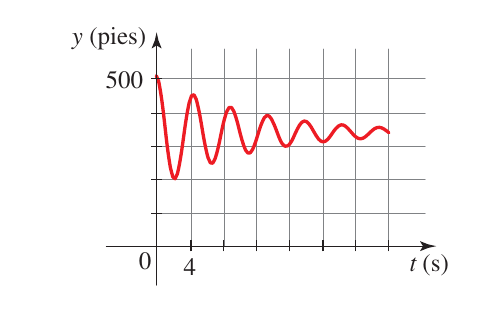
\includegraphics[width=0.52\textwidth]{fig_p06_97.png}\end{center}
\end{quote}

\begin{paso}{Paso 1 --- Leer la gráfica de $h$}
\textbf{Qué hago:} describo: $h(0)=500$ pies, la altura cae rápido hasta el primer punto más bajo, luego oscila con rebotes cada vez menores y se estabiliza en una altura intermedia.

\textbf{¿De dónde sale?} De la figura: la curva parte del valor 500 en $t=0$ y las oscilaciones se van amortiguando.

\textbf{¿Por qué?} La altura es la salida de la función; los picos y valles sucesivos son los rebotes de la cuerda elástica, que pierden amplitud hasta que Luisa queda colgando.
\end{paso}

\begin{paso}{Paso 2 --- Identificar qué cambia al bajar el puente 100 pies}
\textbf{Qué hago:} el salto es el mismo movimiento, pero medido desde un punto de partida 100 pies más bajo, así que toda altura disminuye en 100.

\textbf{¿De dónde sale?} Del enunciado: $500-400=100$ pies de diferencia entre los dos puentes.

\textbf{¿Por qué?} La cuerda y el rebote no cambian; solo cambia el nivel de referencia, y eso afecta la \emph{salida} de la función, no el tiempo.
\end{paso}

\begin{paso}{Paso 3 --- Escribir la transformación y trazar}
\textbf{Qué hago:} $H(t)=h(t)-100$: la gráfica de $H$ es la de $h$ desplazada 100 pies hacia abajo, empezando en $H(0)=400$.

\textbf{¿De dónde sale?} Del paso 2, con la regla $y=f(x)-c$ y $c=100$.

\textbf{¿Por qué?} Regla de desplazamiento vertical: restar una constante a la salida baja la gráfica esa cantidad sin deformarla.

\begin{center}
\begin{tikzpicture}
\begin{axis}[axis lines=middle, xlabel={$t$ (s)}, ylabel={altura (pies)},
  xmin=-0.5,xmax=14, ymin=0,ymax=560, width=11cm,height=6cm,
  grid=both, grid style={gray!20}, ytick={0,100,...,500},
  legend style={font=\small, at={(0.98,0.98)}, anchor=north east}]
  \addplot[thick,blue,domain=0:13,samples=300]{280+220*exp(-0.25*x)*cos(deg(1.6*x))};
  \addlegendentry{$h(t)$ (puente de 500 pies)}
  \addplot[thick,red,domain=0:13,samples=300]{180+220*exp(-0.25*x)*cos(deg(1.6*x))};
  \addlegendentry{$H(t)=h(t)-100$}
\end{axis}
\end{tikzpicture}\\
{\small Esquema: la curva roja es la azul bajada 100 pies; solo importa el desplazamiento vertical.}
\end{center}
\end{paso}

\begin{resp}
\textbf{a)} Luisa parte de 500 pies, cae rápidamente hasta el punto más bajo del salto, rebota varias veces con oscilaciones de amplitud decreciente y termina colgando a una altura constante.\\
\textbf{b)} La misma gráfica trasladada 100 pies hacia abajo: empieza en 400 pies y todos los picos y valles bajan 100 pies.\\
\textbf{c)} Un \textbf{desplazamiento vertical de 100 pies hacia abajo}: $\;H(t)=h(t)-100$.
\end{resp}

\end{document}
